\newpage{\pagestyle{empty}\cleardoublepage}
\newpage{\pagestyle{empty}\cleardoublepage}
\newpage
\vspace*{\fill}
    \begin{center}
      \thispagestyle{empty} \vspace*{0cm} \textbf{\huge
Introducci\'{o}n}
    \end{center}
    \vspace*{\fill}
\newpage{\pagestyle{empty}\cleardoublepage}
\chapter{Visi\'{o}n de la aplicaci\'{o}n}
\section{Descripci\'{o}n general}


Se desea desarrollar una aplicaci\'{o}n para el sector de la compraventa y alquiler de viviendas, la cual permit\'{a} un acceso r\'{a}pido y p\'{u}blico del listado de anuncios que se hayan publicado. \\

Los usuarios visitantes podr\'{a}n consultar anuncios, list\'{a}ndolos, busc\'{a}ndolos de forma global o filtrando por tipo. Se les mostrar\'{a} tambi\'{e}n un listado de comentarios sobre cada anuncio.

Un usuario visitante podr\'{a} registrarse en el sistema, iniciar sesi\'{o}n y acceder a m\'{a}s opciones, adem\'{a}s de las comentadas para los usuarios visitantes. Se podr\'{a} ver su propio perfil, donde el se podr\'{a}n editar sus datos personales y de contacto y un listado de peticiones sobre sus anuncios en vigor. Las gestiones de estas peticiones ser\'{a}n editables desde el mismo punto de perfil, as\'{i} como ofrecer la misma posibilidad de crear nuevos anuncios y consultar y editar los suyos propios. A las peticiones aceptadas se les enviará autom\'{a}ticamente un mensaje al correo electr\'{o}nico con la confirmaci\'{o}n del anunciante.

A diferencia de los usuarios visitantes, los usuarios registrados en el sistema podr\'{a}n comentar y valorar aquellos anuncios que consulten, as\'{i} como realizar peticiones a los anunciantes sobre aquellos en los que est\'{e}n interesados.





El usuario visitante podr\'{a} buscar globalmente en el sistema a trav\'{e}s de un buscador global, as\'{i} como ver de forma ordenada y paginada el listado global de anuncios, en lo posible filtrado seg\'{u}n el tipo de anuncio (en principio compraventa o alquiler) y su tipo de vivienda (en principio casa o piso). Al usuario logado en el sistema se le permitir\'{a} acceder a su perfil desde el navegador principal. Al Administrador, adem\'{a}s, se le proporcionar\'{a} una v\'{i}a de acceso a la zona de gesti\'{o}n.


\begin{figure}[h]
\centering
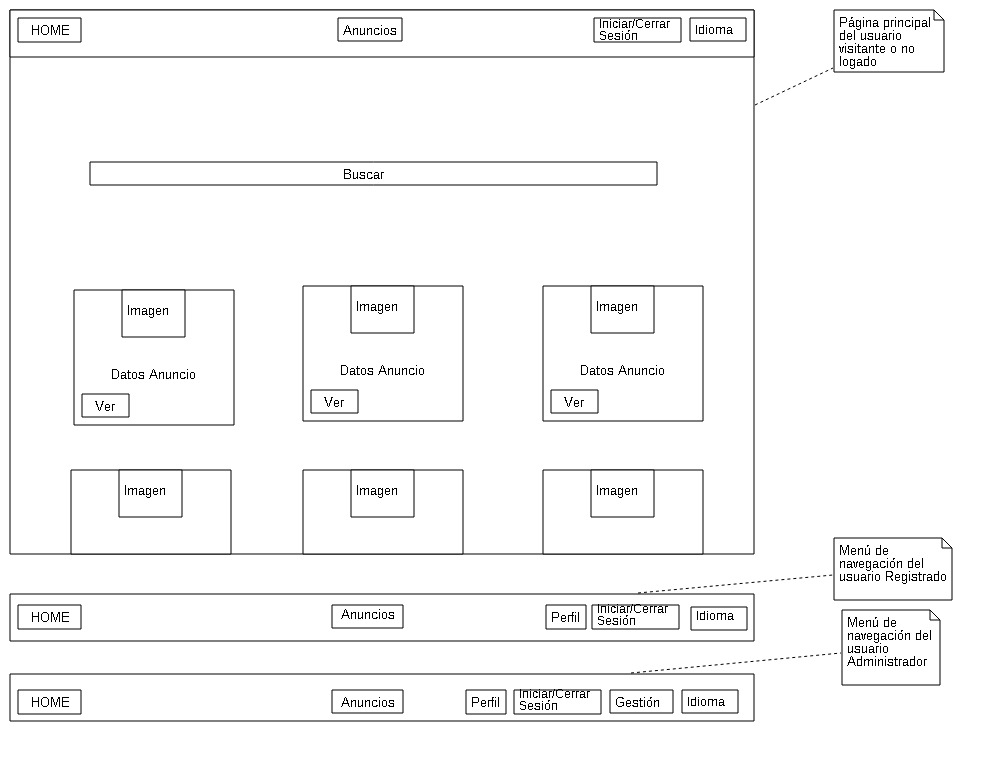
\includegraphics[width=.9\textwidth]{Img/VisionAplicacion/vision_1.jpg}
\end{figure}

Los usuarios que quieran publicar un anuncio deber\'{a}n registrarse y logarse en el sistema. En la alta del anuncio el usuario decidir\'{a} si quiere ofrecer una venta o alquiler, su precio, metros cuadrados, descripci\'{o}n y aportar fotos. Del mismo modo, se proveer\'{a} a los usuarios de la posibilidad de modificar y retirar sus anuncios. Por otro lado, los usuarios registrados podr\'{a}n enviar mensajes privados a otros a trav\'{e}s de los anuncios que se asocien, de forma que siempre exitir\'{a} un v\'{i}nculo entre hilo de mensajes y anuncio de compra, venta o alquiler. Esto compondr\'{a} un sistema de mensajes privados completo.

Los usuarios podr\'{a}n comentar los anuncios de otros usuarios y valorarlos, de tal forma que se mostrar\'{a} la valoraci\'{o}n de un usuario y la valoraci\'{o}n media (entre 0 y 10).


Del usuario administrador se espera que se pueda realizar las mismas funciones que un usuario registrado, aparte de sus tareas de administraci\'{o}n, como puedan ser la gesti\'{o}n de usuarios, anuncios y comentarios, de forma que si alg\'{u}n comentario o anuncio fuera ofensivo, \'{e}ste lo borrar\'{i}a y bloquear\'{i}a al usuario.

En el registro de usuarios, se enviar\'{a} un mensaje de confirmaci\'{o}n al usuario reci\'{e}n registrado para poder activar su cuenta. En caso de no haber activado la cuenta, el usuario no podr\'{a} acceder al sistema. 

\section{Soluci\'{o}n Propuesta}
A continuaci\'{o}n se listar\'{a}n los siguientes cap\'{i}tulos de esta documentaci\'{o}n, en los cuales se recoger\'{a}n las diferentes subsoluciones, adentr\'{a}ndose en diferentes capas o niveles pertenecientes al an\'{a}lisis, dise\~{n}o e implementaci\'{o}n.
\begin{enumerate}
\item An\'{a}lisis
\begin{enumerate}
\item Diagrama de Casos de Uso
\item Descripci\'{o}n de los Casos de Uso.
\item Diagrama del Modelo de Dominio.
\item Diagramas de Secuencia del Sistema y Contratos.
\end{enumerate}
\item Dise\~{n}o
\begin{enumerate}
\item Diagramas de Secuencia.
\item Diagrama de Clase.
\item Test.
\end{enumerate}

\end{enumerate}